%%**************************************************************
%% Vorlage fuer Bachelorarbeiten (o.ä.) der DHBW
%%
%% Autor: Tobias Dreher, Yves Fischer
%% Datum: 06.07.2011
%%
%% Autor: Michael Gruben
%% Datum: 15.05.2013
%%
%% Autor: Markus Barthel
%% Datum: 22.08.2014
%%**************************************************************

%!TEX root = ../dokumentation.tex

%
% Nahezu alle Einstellungen koennen hier getaetigt werden
%

\RequirePackage[l2tabu, orthodox]{nag}	% weist in Commandozeile bzw. log auf veraltete LaTeX Syntax hin

\documentclass[%
	pdftex,
	oneside,			% Einseitiger Druck.
	12pt,				% Schriftgroesse
	parskip=half,		% Halbe Zeile Abstand zwischen Absätzen.
%	topmargin = 10pt,	% Abstand Seitenrand (Std:1in) zu Kopfzeile [laut log: unused]
	headheight = 12pt,	% Höhe der Kopfzeile
%	headsep = 30pt,	% Abstand zwischen Kopfzeile und Text Body  [laut log: unused]
	headsepline,		% Linie nach Kopfzeile.
	footsepline,		% Linie vor Fusszeile.
	footheight = 16pt,	% Höhe der Fusszeile
	abstracton,		% Abstract Überschriften
	DIV=calc,		% Satzspiegel berechnen
	BCOR=8mm,		% Bindekorrektur links: 8mm
	headinclude=false,	% Kopfzeile nicht in den Satzspiegel einbeziehen
	footinclude=false,	% Fußzeile nicht in den Satzspiegel einbeziehen
	listof=totoc,		% Abbildungs-/ Tabellenverzeichnis im Inhaltsverzeichnis darstellen
	toc=bibliography,	% Literaturverzeichnis im Inhaltsverzeichnis darstellen
]{scrreprt}	% Koma-Script report-Klasse, fuer laengere Bachelorarbeiten alternativ auch: scrbook

% Einstellungen laden
\usepackage{xstring}
\usepackage[utf8]{inputenc}
\usepackage[T1]{fontenc}

\newcommand{\einstellung}[1]{%
  \expandafter\newcommand\csname #1\endcsname{}
  \expandafter\newcommand\csname setze#1\endcsname[1]{\expandafter\renewcommand\csname#1\endcsname{##1}}
}
\newcommand{\langstr}[1]{\einstellung{lang#1}}

\einstellung{martrikelnr}
\einstellung{titel}
\einstellung{kurs}
\einstellung{datumAbgabe}
\einstellung{firma}
\einstellung{firmenort}
\einstellung{abgabeort}
\einstellung{abschluss}
\einstellung{studiengang}
\einstellung{dhbw}
\einstellung{betreuer}
\einstellung{gutachter}
\einstellung{zeitraum}
\einstellung{arbeit}
\einstellung{autor}
\einstellung{sprache}
\einstellung{schriftart}
\einstellung{seitenrand}
\einstellung{kapitelabstand}
\einstellung{spaltenabstand}
\einstellung{zeilenabstand}
\einstellung{zitierstil}
 % verfügbare Einstellungen
%%%%%%%%%%%%%%%%%%%%%%%%%%%%%%%%%%%%%%%%%%%%%%%%%%%%%%%%%%%%%%%%%%%%%%%%%%%%%%%
%                                   Einstellungen
%
% Hier können alle relevanten Einstellungen für diese Arbeit gesetzt werden.
% Dazu gehören Angaben u.a. über den Autor sowie Formatierungen.
%
%
%%%%%%%%%%%%%%%%%%%%%%%%%%%%%%%%%%%%%%%%%%%%%%%%%%%%%%%%%%%%%%%%%%%%%%%%%%%%%%%


%%%%%%%%%%%%%%%%%%%%%%%%%%%%%%%%%%%% Sprache %%%%%%%%%%%%%%%%%%%%%%%%%%%%%%%%%%%
%% Aktuell sind Deutsch und Englisch unterstützt.
%% Es werden nicht nur alle vom Dokument erzeugten Texte in
%% der entsprechenden Sprache angezeigt, sondern auch weitere
%% Aspekte angepasst, wie z.B. die Anführungszeichen und
%% Datumsformate.
\setzesprache{en} % oder en
%%%%%%%%%%%%%%%%%%%%%%%%%%%%%%%%%%%%%%%%%%%%%%%%%%%%%%%%%%%%%%%%%%%%%%%%%%%%%%%%

%%%%%%%%%%%%%%%%%%%%%%%%%%%%%%%%%%% Angaben  %%%%%%%%%%%%%%%%%%%%%%%%%%%%%%%%%%%
%% Die meisten der folgenden Daten werden auf dem
%% Deckblatt angezeigt, einige auch im weiteren Verlauf
%% des Dokuments.
\setzetitel{Datenbank Implementationen}
%\setzetitel{Logfileanalyse mit Apache{\textsuperscript{TM}} Hadoop\textsuperscript{{\textregistered}} MapReduce}
\setzedatumAbgabe{April 2017}
\setzeabgabeort{Stuttgart}
%\setzeabschluss{Abschluss}
\setzestudiengang{Angewandte Informatik}
\setzedhbw{Stuttgart}
%\setzegutachter{nothing}
%\setzezeitraum{2 Wochen}
\setzearbeit{Das E-Book.}
\setzeautor{IT14C}
%%%%%%%%%%%%%%%%%%%%%%%%%%%%%%%%%%%%%%%%%%%%%%%%%%%%%%%%%%%%%%%%%%%%%%%%%%%%%%%%

%%%%%%%%%%%%%%%%%%%%%%%%%%%% Literaturverzeichnis %%%%%%%%%%%%%%%%%%%%%%%%%%%%%%
%% Bei Fehlern während der Verarbeitung bitte in ads/header.tex bei der
%% Einbindung des Pakets biblatex (ungefähr ab Zeile 110,
%% einmal für jede Sprache), biber in bibtex ändern.
\newcommand{\ladeliteratur}{%
\addbibresource{bibliographie.bib}
%\addbibresource{weitereDatei.bib}
}
%% Zitierstil
%% siehe: http://ctan.mirrorcatalogs.com/macros/latex/contrib/biblatex/doc/biblatex.pdf (3.3.1 Citation Styles)
%% mögliche Werte z.B numeric-comp, alphabetic, authoryear
\setzezitierstil{authoryear}
%%%%%%%%%%%%%%%%%%%%%%%%%%%%%%%%%%%%%%%%%%%%%%%%%%%%%%%%%%%%%%%%%%%%%%%%%%%%%%%%

%%%%%%%%%%%%%%%%%%%%%%%%%%%%%%%%% Layout %%%%%%%%%%%%%%%%%%%%%%%%%%%%%%%%%%%%%%%
%% Verschiedene Schriftarten
% laut nag Warnung: palatino obsolete, use mathpazo, helvet (option scaled=.95), courier instead
\setzeschriftart{lmodern} % palatino oder goudysans, lmodern, libertine

%% Paket um Textteile drehen zu können
%\usepackage{rotating}
%% Paket um Seite im Querformat anzuzeigen
%\usepackage{lscape}

%% Seitenränder
\setzeseitenrand{2.5cm}

%% Abstand vor Kapitelüberschriften zum oberen Seitenrand
\setzekapitelabstand{20pt}

%% Spaltenabstand
\setzespaltenabstand{10pt}
%%Zeilenabstand innerhalb einer Tabelle
\setzezeilenabstand{1.5}
%%%%%%%%%%%%%%%%%%%%%%%%%%%%%%%%%%%%%%%%%%%%%%%%%%%%%%%%%%%%%%%%%%%%%%%%%%%%%%%%

%%%%%%%%%%%%%%%%%%%%%%%%%%%%% Verschiedenes  %%%%%%%%%%%%%%%%%%%%%%%%%%%%%%%%%%%
%% Farben (Angabe in HTML-Notation mit großen Buchstaben)
\newcommand{\ladefarben}{%
	\definecolor{LinkColor}{HTML}{00007A}
	\definecolor{ListingBackground}{HTML}{FCFAFB}
}
%% Mathematikpakete benutzen (Pakete aktivieren)
\usepackage{amsmath}
\usepackage{amssymb}

%% Programmiersprachen Highlighting (Listings)
\newcommand{\listingsettings}{%
	\lstset{%
		language=C,			% Standardsprache des Quellcodes
		numbers=left,			% Zeilennummern links
		stepnumber=1,			% Jede Zeile nummerieren.
		numbersep=5pt,			% 5pt Abstand zum Quellcode
		numberstyle=\tiny,		% Zeichengrösse 'tiny' für die Nummern.
		breaklines=true,		% Zeilen umbrechen wenn notwendig.
		breakautoindent=true,	% Nach dem Zeilenumbruch Zeile einrücken.
		postbreak=\space,		% Bei Leerzeichen umbrechen.
		tabsize=2,				% Tabulatorgrösse 2
		basicstyle=\ttfamily\footnotesize, % Nichtproportionale Schrift, klein für den Quellcode
		showspaces=false,		% Leerzeichen nicht anzeigen.
		showstringspaces=false,	% Leerzeichen auch in Strings ('') nicht anzeigen.
		extendedchars=true,		% Alle Zeichen vom Latin1 Zeichensatz anzeigen.
		captionpos=b,			% sets the caption-position to bottom
		backgroundcolor=\color{ListingBackground}, % Hintergrundfarbe des Quellcodes setzen.
		xleftmargin=0pt,		% Rand links
		xrightmargin=0pt,		% Rand rechts
		frame=single,			% Rahmen an
		frameround=ffff,
		rulecolor=\color{darkgray},	% Rahmenfarbe
		fillcolor=\color{ListingBackground},
		keywordstyle=\color[rgb]{0.133,0.133,0.6}\bfseries,
		commentstyle=\color{Sepia},
		stringstyle=\color{red}
	}
}
%%%%%%%%%%%%%%%%%%%%%%%%%%%%%%%%%%%%%%%%%%%%%%%%%%%%%%%%%%%%%%%%%%%%%%%%%%%%%%%%

%%%%%%%%%%%%%%%%%%%%%%%%%%%%%%%% Eigenes %%%%%%%%%%%%%%%%%%%%%%%%%%%%%%%%%%%%%%%
%% Hier können Ergänzungen zur Präambel vorgenommen werden (eigene Pakete, Einstellungen)

% xcolor muss mit optionen vor pdfpages geladen werden
\usepackage[usenames,dvipsnames,table,xcdraw]{xcolor} 	%xcolor für HTML-Notation

\usepackage{pdfpages}
 % lese Einstellungen

\newcommand{\iflang}[2]{%
  \IfStrEq{\sprache}{#1}{#2}{}
}

\langstr{abkverz}
\langstr{anhang}
\langstr{glossar}
\langstr{deckblattabschlusshinleitung}
\langstr{artikelstudiengang}
\langstr{studiengang}
\langstr{anderdh}
\langstr{von}
\langstr{dbbearbeitungszeit}
\langstr{dbmatriknr}
\langstr{dbkurs}
\langstr{dbfirma}
\langstr{dbbetreuer}
\langstr{dbgutachter}
\langstr{sperrvermerk}
\langstr{erklaerung}
\langstr{abstract}
\langstr{listingname}
\langstr{listlistingname}
\langstr{listingautorefname}
 % verfügbare Strings
\input{lang/\sprache} % Übersetzung einlesen

% Einstellung der Sprache des Paketes Babel und der Verzeichnisüberschriften
\iflang{de}{\usepackage[english, ngerman]{babel}}
\iflang{en}{\usepackage[ngerman, english]{babel}} 


%%%%%%% Package Includes %%%%%%%

\usepackage[margin=\seitenrand,foot=1cm]{geometry}	% Seitenränder und Abstände
\usepackage[activate]{microtype} %Zeilenumbruch und mehr
\usepackage[onehalfspacing]{setspace}
\usepackage{makeidx}
\usepackage[autostyle=true,german=quotes]{csquotes}
\usepackage{tabularx}
\usepackage{longtable}
\usepackage{multirow}
\usepackage{enumitem}	% mehr Optionen bei Aufzählungen
\usepackage{graphicx}
%\usepackage[usenames,dvipsnames,table,xcdraw]{xcolor} 	%xcolor für HTML-Notation
\usepackage{float}
\usepackage{array}
\usepackage{calc}		% zum Rechnen (Bildtabelle in Deckblatt)
\usepackage[right]{eurosym}
\usepackage{wrapfig}
\usepackage{pgffor} % für automatische Kapiteldateieinbindung
\usepackage[perpage, hang, multiple, stable]{footmisc} % Fussnoten
%\usepackage[nohyperlinks]{acronym} % falls gewünscht kann die Option footnote eingefügt werden, dann wird die Erklärung nicht inline sondern in einer Fußnote dargestellt
\usepackage{acronym}

\usepackage{listings}

% Eigene zusätzliche packages
\usepackage{xfrac}
\usepackage{tikz}
\usepackage{subcaption}
%\usepackage[leqno]{amsmath}
%\usepackage{remreset}

% Wurzel mit schießendem Strich am ende
% New definition of square root: % it renames \sqrt as \oldsqrt
\let\oldsqrt\sqrt % it defines the new \sqrt in terms of the old one 
\def\sqrt{\mathpalette\DHLhksqrt} \def\DHLhksqrt#1#2{
\setbox0=\hbox{$#1\oldsqrt{#2\,}$}\dimen0=\ht0 \advance\dimen0-0.2\ht0 \setbox2=\hbox{\vrule height\ht0 depth -\dimen0}{\box0\lower0.4pt\box2}}

%\makeatletter
%\@removefromreset{equation}{chapter}
%\makeatother
%\renewcommand*{\theequation}{\arabic{equation}}

% eine Kommentarumgebung "k" (Handhabe mit \begin{k}<Kommentartext>\end{k},
% Kommentare werden rot gedruckt). Wird \% vor excludecomment{k} entfernt,
% werden keine Kommentare mehr gedruckt.
\usepackage{comment}
\specialcomment{k}{\begingroup\color{red}}{\endgroup}
%\excludecomment{k}


%%%%%% Configuration %%%%%

%% Anwenden der Einstellungen

\usepackage{\schriftart}
\ladefarben{}

% Titel, Autor und Datum
\title{\titel}
\author{\autor}
\date{\datum}

% PDF Einstellungen
\usepackage[%
	pdftitle={\titel},
	pdfauthor={\autor},
	pdfsubject={\arbeit},
	pdfcreator={pdflatex, LaTeX with KOMA-Script},
	pdfpagemode=UseOutlines, 		% Beim Oeffnen Inhaltsverzeichnis anzeigen
	pdfdisplaydoctitle=true, 		% Dokumenttitel statt Dateiname anzeigen.
	pdflang={\sprache}, 			% Sprache des Dokuments.
]{hyperref}

% (Farb-)einstellungen für die Links im PDF
\hypersetup{%
	colorlinks=true, 		% Aktivieren von farbigen Links im Dokument
	linkcolor=LinkColor, 	% Farbe festlegen
	citecolor=LinkColor,
	filecolor=LinkColor,
	menucolor=LinkColor,
	urlcolor=LinkColor,
	linktocpage=true, 		% Nicht der Text sondern die Seitenzahlen in Verzeichnissen klickbar
	bookmarksnumbered=true 	% Überschriftsnummerierung im PDF Inhalt anzeigen.
}
% Workaround um Fehler in Hyperref, muss hier stehen bleiben
\usepackage{bookmark} %nur ein latex-Durchlauf für die Aktualisierung von Verzeichnissen nötig

% Schriftart in Captions etwas kleiner
\addtokomafont{caption}{\small}

% % Literaturverweise (sowohl deutsch als auch englisch)
% \iflang{de}{%
% \usepackage[
% 	backend=bibtex,		% empfohlen. Falls biber Probleme macht: bibtex
% 	bibwarn=true,
% 	bibencoding=utf8,	% wenn .bib in utf8, sonst ascii
% 	sortlocale=de_DE,
% 	style=\zitierstil,
% 	backref=true
% ]{biblatex}
% }
% \iflang{en}{%
% \usepackage[
% 	backend=bibtex,		% empfohlen. Falls biber Probleme macht: bibtex
% 	bibwarn=true,
% 	bibencoding=utf8,	% wenn .bib in utf8, sonst ascii
% 	sortlocale=en_US,
% 	style=\zitierstil,
% ]{biblatex}
% }

% % Mehr Platz zwischen einzelnen Items im Literaturverzeichnis bei Verwendung von authoryear
% \setlength{\bibitemsep}{\baselineskip}
% \DeclareNameAlias{sortname}{last-first}
% 
% \ladeliteratur{}
\usepackage{apacite}
% Glossar
\usepackage[nonumberlist,toc]{glossaries}

%%%%%% Additional settings %%%%%%

% Hurenkinder und Schusterjungen verhindern
% http://projekte.dante.de/DanteFAQ/Silbentrennung
\clubpenalty = 10000 % schließt Schusterjungen aus (Seitenumbruch nach der ersten Zeile eines neuen Absatzes)
\widowpenalty = 10000 % schließt Hurenkinder aus (die letzte Zeile eines Absatzes steht auf einer neuen Seite)
\displaywidowpenalty=10000

% Bildpfad
\graphicspath{{images/}}

% Einige häufig verwendete Sprachen
\lstloadlanguages{PHP,Python,Java,C,C++,bash,XML}
\listingsettings{}
% Umbennung des Listings
\renewcommand\lstlistingname{\langlistingname}
\renewcommand\lstlistlistingname{\langlistlistingname}
\def\lstlistingautorefname{\langlistingautorefname}

% Umlaute ermöglichen in listings
\lstset{literate=
	{á}{{\'a}}1 {é}{{\'e}}1 {í}{{\'i}}1 {ó}{{\'o}}1 {ú}{{\'u}}1
	{Á}{{\'A}}1 {É}{{\'E}}1 {Í}{{\'I}}1 {Ó}{{\'O}}1 {Ú}{{\'U}}1
	{à}{{\`a}}1 {è}{{\`e}}1 {ì}{{\`i}}1 {ò}{{\`o}}1 {ù}{{\`u}}1
	{À}{{\`A}}1 {È}{{\'E}}1 {Ì}{{\`I}}1 {Ò}{{\`O}}1 {Ù}{{\`U}}1
	{ä}{{\"a}}1 {ë}{{\"e}}1 {ï}{{\"i}}1 {ö}{{\"o}}1 {ü}{{\"u}}1
	{Ä}{{\"A}}1 {Ë}{{\"E}}1 {Ï}{{\"I}}1 {Ö}{{\"O}}1 {Ü}{{\"U}}1
	{â}{{\^a}}1 {ê}{{\^e}}1 {î}{{\^i}}1 {ô}{{\^o}}1 {û}{{\^u}}1
	{Â}{{\^A}}1 {Ê}{{\^E}}1 {Î}{{\^I}}1 {Ô}{{\^O}}1 {Û}{{\^U}}1
	{œ}{{\oe}}1 {Œ}{{\OE}}1 {æ}{{\ae}}1 {Æ}{{\AE}}1 {ß}{{\ss}}1
	{ç}{{\c c}}1 {Ç}{{\c C}}1 {ø}{{\o}}1 {å}{{\r a}}1 {Å}{{\r A}}1
	{€}{{\EUR}}1 {£}{{\pounds}}1
}

% Weitere Keyword Highlights
\lstset{
	emph=[1]{ 
	    mkdir, jps, sudo, wget, mv, chown, su, adduser, addgroup, grep, sort, print, max, WARNING
    },
    emphstyle=[1]{\color[rgb]{0.133,0.133,0.6}},
    emph=[2]{
	    LFAConfiguration, Driver, Set, Exception, Configuration, FileInputFormat, FileOutputFormat, Job, Path, Text, IntWritable, Mapper, Matcher, Pattern, PatternMapper, Logger, Level, Context, IOException, InterruptedException, Reducer, CountReducer, TextInputFormat, TextOutputFormat, RecordReader, PDFInputFormat, PDFLineRecordReader, InputSplit, TaskAttemptContext, JobContext, CharSequence
    },
    emphstyle=[2]{\color[HTML]{006400}},
    emph=[3]{
	    String, int, Object, Iterable, boolean, Class, float
    },
    emphstyle=[3]{\color{Mulberry}}
}

% Abstände in Tabellen
\setlength{\tabcolsep}{\spaltenabstand}
\renewcommand{\arraystretch}{\zeilenabstand}


\makeglossaries
%!TEX root = ../dokumentation.tex

%
% vorher in Konsole folgendes aufrufen:
%	makeglossaries makeglossaries dokumentation.acn && makeglossaries dokumentation.glo
%

%
% Glossareintraege --> referenz, name, beschreibung
% Aufruf mit \gls{...}
%
\newglossaryentry{Glossareintrag}{name={Glossareintrag},plural={Glossareinträge},description={Ein Glossar beschreibt verschiedenste Dinge in kurzen Worten}}

\newglossaryentry{Commodity-Hardware}{name={Commodity-Hardware},description={\flqq Computer hardware that is affordable and easy to obtain. Typically it is a low-performance system that is IBM PC-compatible and is capable of running Microsoft Windows, Linux, or MS-DOS without requiring any special devices or equipment.\frqq\footcite{Beal.2015}}}

\newglossaryentry{Git}{name={Git},plural={Git},description={Git ist ein kostenloses System zur Versionskontrolle für kleine wie auch sehr große Projekte. ({\url{http://git-scm.com/}})}}

\newglossaryentry{NetBeans}{name={NetBeans},plural={NetBeans},description={The Smarter and Faster Way to Code Quickly and easily develop desktop, mobile and web applications with Java, HTML5, PHP, C/C++ and more. NetBeans IDE is FREE, open source, and has a worldwide community of users and developers. ({\url{https://netbeans.org}})}}

\newglossaryentry{Maven}{name={Maven},plural={Maven},description={Apache Maven is a software project management and comprehension tool. Based on the concept of a project object model (POM), Maven can manage a project’s build, reporting and documentation from a central piece of information. \\ ({\url{http://maven.apache.org/}})}}

\newglossaryentry{Nagios}{name={Nagios},plural={Nagios},description={Nagios Is The Industry Standard In IT Infrastructure Monitoring. Achieve instant awareness of IT infrastructure problems, so downtime doesn't adversely affect your business. Nagios offers complete monitoring and alerting for servers, switches, applications, and services. \\ ({\url{https://www.nagios.org}})}}

\newglossaryentry{Zabbix}{name={Zabbix},plural={Zabbix},description={Zabbix is the ultimate enterprise-level software designed for real-time monitoring of millions of metrics collected from tens of thousands of servers, virtual machines and network devices. Zabbix is Open Source and comes at no cost. \\ ({\url{http://www.zabbix.com}})}}

\newglossaryentry{Bootstrapping}{name={Bootstrapping},description={\flqq The computer term bootstrap began as a metaphor in the 1950s. In computers, pressing a bootstrap button caused a hardwired program to read a bootstrap program from an input unit. The computer would then execute the bootstrap program, which caused it to read more program instructions. It became a self-sustaining process that proceeded without external help from manually entered instructions. As a computing term, bootstrap has been used since at least 1953.\frqq\footcite[S. 1273]{Buchholz.1953}}}

\newglossaryentry{Generic}{name={Generic},plural={Generics},description={Ein Interface oder eine Klasse kann mit einem oder mehreren Parametern, den sog. Generics, definiert werden, welche zusätzliche Typangaben enthalten. Diese werden in spitzen Klammern notiert. Generics führen implizit einen Typumwandlung durch, welcher ohne Generics explizit erfolgen müsste\footcite[Vgl.][S. 4 f.]{Naftalin.2006}}}

\newglossaryentry{Plugin}{name={Plugin},plural={Plugins},description={\flqq Zusatzprogramm, welches über eine vordefinierte Schnittstelle in ein Basisprogramm eingebunden wird und dessen Funktionsumfang erweitert. [...] [Stammen] oftmals von anderen Herstellern als das Basisprogramm. [...] Plug-ins sind oft aus eigenständigen Programmen entstanden und können deshalb [...] i.d.R. auch ohne das Basisprogramm verwendet werden\frqq\footcite[]{Lackes.2015}}}

\usepackage{enumitem}
\usepackage[table,xcdraw]{xcolor}

\begin{document}

	% Deckblatt
	\begin{spacing}{1}
		%!TEX root = ../dokumentation.tex

\begin{titlepage}
	\begin{longtable}{p{8.2cm} p{5.4cm}}
%		{\raisebox{\ht\strutbox-\totalheight}{
\includegraphics[scale=3]{images/firma-deckblatt.jpg}}} &
		{\raisebox{\ht\strutbox-\totalheight}{
\includegraphics[height=2.5cm]{images/dhbw.png}}}
	\end{longtable}
	\enlargethispage{20mm}
	\begin{center}
		\vspace*{12mm}	{\LARGE\textbf \titel }\\
		\vspace*{12mm}
		\vspace*{12mm}	{\large\textbf \arbeit}\\
		%\vspace*{12mm}	\langdeckblattabschlusshinleitung\\
		\vspace*{12mm}
		%\vspace*{3mm}		{\textbf \abschluss}\\
		%\vspace*{12mm}	\langartikelstudiengang{} \langstudiengang{} \studiengang\\
    \vspace*{3mm}		\langanderdh{} \dhbw\\
		\vspace*{12mm}	\langvon\\
		\vspace*{3mm}		{\large\textbf \autor}\\
		\vspace*{12mm}	\datumAbgabe\\
	\end{center}
	\vfill
\end{titlepage}

	\end{spacing}
	\newpage
	\pagestyle{plain}	

	% Inhaltsverzeichnis
	\begin{spacing}{1.1}
		\begingroup
			\setcounter{tocdepth}{2}
			\tableofcontents
			\clearpage
		\endgroup
	\end{spacing}
	\newpage

	\pagenumbering{arabic}
	
	\pagestyle{headings}		% Kolumnentitel im Kopf, Seitenzahlen im Fuß

	% Vorlage
	\chapter{Riak}
Riak is available in two versions. There is Riak TS for time series data and Riak KV. The chapter about Riak concentrates on Riak KV (further "Riak").
\section{Introduction into Riak}
The following chapter provides an introduction into Riak and its main features. 
\subsection{General Information}
Riak is a distributed key-value NoSQL database designed for high availability use cases. As long as the client can reach one Riak node the data is available. The reason is that data is saved across multiple servers. How the clustering works will be shown in the next chapter. \cite{Basho.06.04.2017}
\\
Riak is available for different operating systems, e.g. Ubuntu, CentOS or Mac OS X but not for Windows. The installation is straight-forward because you just have to download a package from the official website and install the package. \cite{Basho.06.04.2017}
\\ 
As data is saved across multiple servers even hardware or network failures can be handled by Riak. If you need more space for your data new servers can be added easily. By adding new servers the scalability is nearly linear which is very impressive. \cite{Basho.06.04.2017}
\\
Data is saved in buckets. A bucket in Riak can be compared with a table in a SQL-database. \cite{Basho.06.04.2017}
\\ 
Now if you have a look on the CAP-Theorem one can say that Riak definitely concentrates on "A" and "P" - Availability and Partition Tolerance. If your system needs high availability and you can not accept downtime Riak is probably the best solution. Another feature of Riak is its latency: since the CRUD-operations do not involve complex joins the requests are serviced promptly. \cite{Basho.06.04.2017}
\\
On the other hand if your system needs a high consistency of the data Riak is not the right choice. \cite{Basho.06.04.2017}
\subsection{Riak Clustering}
The high availability of Riak can only be achieved by the Riak clustering. The official website of Riak recommends that there should be at least five nodes in one cluster. A node is a server in production environment - during the development of the software there can be more than one node on a server. \cite{Basho.06.04.2017}
\\
All nodes have the same responsibility, this means there is no kind of master-node which has special tasks. \cite{Basho.06.04.2017}

The clustering is visible in the logo of Riak as well. There is one node and three lines to other nodes which symbolize the replication of data:
\begin{figure}[h!]
	\centering
	
\includegraphics[width=3.0in]{riak_logo.png}
	\caption[Riak Logo \protect\cite{Basho.06.04.2017}]{Riak Logo \protect\cite{Basho.06.04.2017}}
	\label{Riak Logo}
\end{figure}

\subsubsection{Automatic re-distribution of data}
When new servers are added or when machines are removed Riak automatically re-distributes the data with no downtime. Data is spread in the cluster until each node owns the same amount of data. This is why developers do not need to care about where the data is saved. Riak uses consistent hashing to distribute data evenly across the nodes in a cluster. Consistent hashing limits the reshuffling of keys when a hash-table structure is rebalanced. \cite{Basho.06.04.2017}
\subsubsection{Intelligent Replication}
Even if nodes fail the user should be able to read and write data. The replication scheme ensures the availability by setting a replication variable, that specifies the number of nodes on which a value will be replicated. The default number is three which means that each object is replicated three times. If Riak can access one node where the object is replicated it is available for the client. \cite{Basho.06.04.2017}
\\ 
The following picture describes the replication: 
\begin{figure}[h]
	\centering
	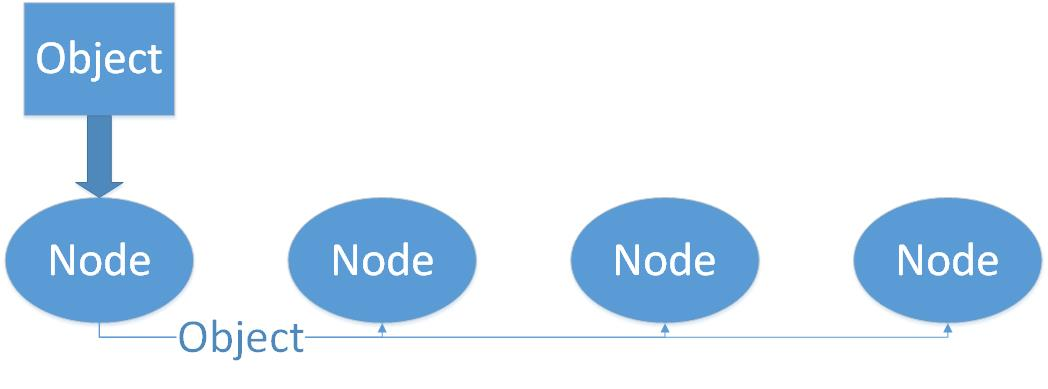
\includegraphics[width=3.0in]{riak_clustering.jpg}
	\caption{Riak Clustering}
	\label{Riak Clustering}
\end{figure}
\section{Open Source vs. Enterprise}

Basho provides five different versions of the Riak KV database, so that the customers always find the perfect configuration for their purpose. The variants are named \textit{Open Source}, \textit{Developer}, \textit{Pro}, \textit{Enterprise} and \textit{Enterprise Plus}. Every configuration has a different composition of features. Figure \ref{fig:overview} shows a short overview of the versions and the related features.

\begin{figure}[ht]
	\centering
	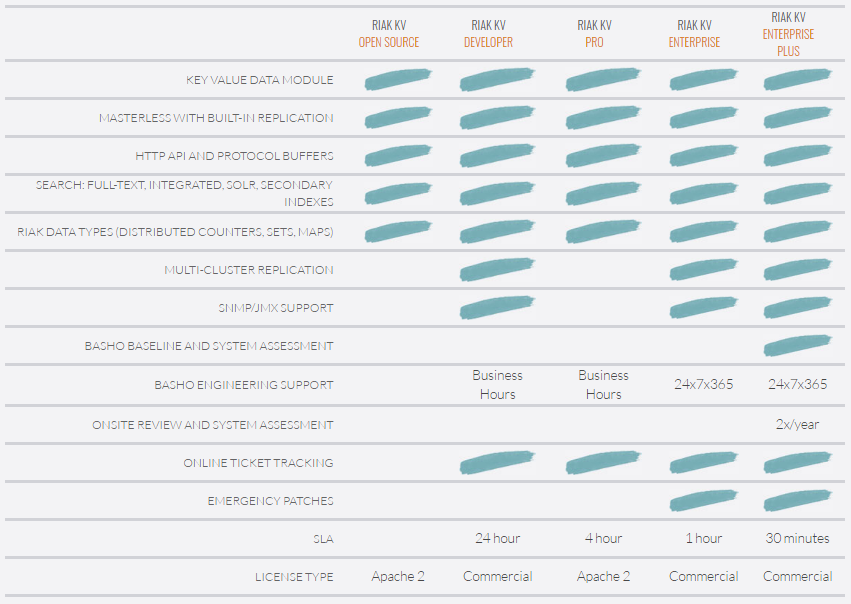
\includegraphics[width=\textwidth]{images/opensource_vs_commercial.png}
	\caption[Overview of different versions of Riak KV \protect\cite{Basho.01.04.2017}]{Overview of different versions of Riak KV \protect\cite{Basho.01.04.2017}}
	\label{fig:overview}
\end{figure}

In the following, every feature is individually viewed and explained in detail.

\newpage

\textbf{Key Value Data Module}\newline
Of course every configuration uses the key value data module developed by Basho.

\textbf{Masterless with Built-In Replication}\newline
All configurations are masterless with an integrated replication. This means that data is replicated automatically on multiple nodes so that the application remains available for both read and write operations. This is the way the database achieves high availability.

\textbf{HTTP API and Protocol Buffers}\newline
Every version works with a simple HTTP API and Protocol Buffers. Protocol Buffers is a method of serializing structured data and is especially useful for storing data. 

\textbf{Search}\newline
All implementations of the Riak KV support an integrated fulltext search and Apache Solr. Apache Solr is a popular open source enterprise search platform  built on Apache Lucene. This means with Apache Solr the user can search the whole database at once.

\textbf{Riak Data Types}\newline
Certainly all versions use the Riak data types which are \textit{Flags}, \textit{Registers}, \textit{Counters}, \textit{Sets} and \textit{Maps}. Flags are similar the same as Boolean, except the values are called \textit{enable} and \textit{disable}. Registers are essentially named binaries like Strings. Flags and Registers are no bucket-level Riak data types. They cannot be used on their own and have to be embedded in Maps. Counters keep track of increments or decrements. Sets are collections of unique binary values. Maps enable the creation of complex, custom data types because all other data types could be embedded.

\textbf{Multi-Cluster Replication}\newline
This feature is just available for the commercial versions of Riak. The data clusters are replicated automatically in several datacenters of the customer. If one cluster fails another one provides the necessary data. 

\textbf{SNMP / JMX Support}\newline
SNMP means \textit{Simple Network Management Protocol} and is an internet-standard protocol for collecting and organizing information about managed devices on IP networks. JMX stands for \textit{Java Management Extensions} and is a Java technology that provides tools for managing und monitoring applications, devices and system objects. Customers that use a commercial configuration of Riak are able to implement these extensions and monitor their database.

\newpage

\textbf{Basho Baseline and System Assessment}\newline
This feature is obtainable just for customers of the Enterprise Plus package. An engineer of the Basho team reviews the whole configuration of the database via remote access before Riak is deployed. 


\textbf{Basho Engineering Support}\newline
The Basho Engineering Support is a simple support hotline. Since the Basho team only provides payed support, this offer is not available for the open source variant. The user has to have an account to contact the support team.


\textbf{Onsite Review and System Assessment}\newline
That system assessment is nearly the same as the previous one. The only difference is that the assessment is not done via remote access, but a team of engineers come to the customer’s location and review the system onsite.

\textbf{Online Ticket Tracking}\newline
The Online Ticket Tracking is a functionality of the account that is needed if you do not use the open source version. In combination with the ability to contact the support team, the user can see the current state of his support ticket.

\textbf{Emergency Patches}\newline
If the customers of the Enterprise versions face a problem with their database, the Basho team provides a patch as soon as possible. 

\textbf{Service Level Agreements}\newline
The Service Level Agreements are between 24 hours and 30 minutes response time after a problem report was sent by the customer. Afterwards the engineering team provides a solution for the problem as soon as possible. 

\textbf{License Type}\newline
The last point of this comparsion is the license type. Riak KV Open Source and Riak KV Pro are available under the open source license Apache 2. The other three configurations use a commercial license.

\newpage
\section{Advantages}
Since Riak is a distributed database there are different advantages making Riak special. Riak focuses on high availability, easy scalability and data safety. This is achieved through the distribution of the database across several nodes. \cite{Basho.01.04.2017}
The main advantages of the distributed approach are:
\begin{itemize}
	\item Installation
	\item Scalability
	\item Availability
	\item Interaction
	\item Error management
\end{itemize}
In the following subsections this concepts will be described in more detail. 
\subsection{Installation}
The installation of Riak is easy and straight forward. Riak is available for various Linux distributions and Mac OS X. There is an Dabian package for Ubuntu, delivered through bashos web page (HTTP://docs.Bashocom/riak/kv/2.2.2/downloads/). This package can be easily installed with Ubuntus package manager. After the setup you are ready to go. With the command \textit{"riak start"} a Riak cluster with one node and the standard settings is started. \cite{Basho.01.04.17c}
\subsection{Scalability}
Riak uses a distributed cluster approach built up of several nodes which makes it highly scalable. If there is a need for higher performance or stability there could be easily added several nodes to the cluster. This can be done even when the database is running. 
Before a node can be added to a cluster it needs to be started with the \textit{"riak start"} command. After the node is running it can be added to a cluster with the \textit{"riak cluster join"} command. \cite{Basho.01.04.17b}
\subsection{Availability}
A special feature of Riak is its high availability Riak uses a masterless system resulting in no single point of failure. If all nodes fail except one this last node will take all of the responsibilities of the other nodes. The cluster gets very slow, but it stays available and responsive.
\subsection{Interaction}
Another unique selling point of Riak is its native HTTP 1.1 API. This API is designed as RESTful Web service. Create, read, update and delete (CRUD) actions can be performed over the corresponding HTTP methods. This makes Riak a very flexible and handy database. 
Besides that Riak guarantees client support for common programming languages like Java, Ruby, Python, C\#, Node.js, PHP, Erlang and Go.  
\subsection{Error management}
If multiple clients can write concurrently, potentially to the same key it is very likely that errors could happen. Therefore Riak has to use an error management. There is an logical approach called vector clock which abstracts the states of a data set on an analogous clock to track the history of updates to value. If the data is corrupted Riak through conflict writes, it can be restored through this mechanism. 
\section{Disadvantages}
As the previous section shows is the distributed approach of Riak a very beneficial and useful. But besides this advantages there are some downsides as well. Several nodes and the masterless concept lead to various problems like:
 \begin{itemize}
 	\item Inconsistency
 	\item Vector-clocks
 	\item No rollbacks
 \end{itemize}
 In the next subsections we dig a little bit deeper in those problems. \cite{FHKoln.01.04.17}
 \subsection{Inconsistency}
 The main problem of highly-available, clustered systems like Riak is the validity of data sets. Due to the fact that there are no ACID transactions data sets can get inconsistent. There is no mechanism guaranteeing the transfer of a consistent state into another. This results in conflicting responses and anomalies which have to be handled.  
 \subsection{Vector-clocks}
 Although the error management concept of Riak is very reasoned the vector-clock system is leading to some difficulties. It is possible that Riak creates different values for an object on various nodes. These values are called siblings. This could lead to inconsistency and conflicts.
 \subsection{No rollbacks}
 Although Riak has a very sophisticated error management system there is no way to completely restore a dataset. This is due to a missing rollback and commit mechanism. This means if you have done any change to the data it is irreversible.  
 \newpage
 \section{Use Cases}
 As you may have noticed, Riak is a quite special database solution. There are several use cases Riak is perfectly suited for. The first one described in here is session data. This means the usage of Riak for storing users and sessions into a Riak database. This data is usually used to save data  about the application’s connection with the user. Therefore it is very important to have this data highly available.
 Another common use case for Riak are chat and messenger applications. Traditional rational databases are not suited for the heterogeneous data messaging applications bring along. Therefore key value databases like Riak are more efficient way to save those data. Furthermore the highly-available, low-latency data architecture of Riak provides a good base for messaging apps which are always available.
 The next point is business continuity. This means applications which should not have a downtime of several minutes. With Riak you can scale an maintain such applications even if the database even if it is running. This is why Riak fits perfectly well in this use case.
 The last point described in this section is the usage of Riak for saving content and documents. This documents are highly unstructured because there are a huge amount of different data like pdf files, log files, emails, chat history, books, articles and videos. With Riak all of this data can be saved in a proper manner. There is no overload of as in a rational database. \cite{Basho.01.04.17}  
 
 To conclude with, Riak is used by several companies in the gaming, retail, telecommunications and transportation area as high available and scalable database. Well known companies which use Riak are Uber, Rovio, Best Buy, Xing and Symantec. \cite{Basho.01.04.17b}
 
 \newpage
\section{Conclusion}
As a conclusion one can say that the feature "CRUD"-Operations via REST is very useful but in newer versions \textbf{C}ross \textbf{O}rigin \textbf{R}esource \textbf{S}haring should be available since you can't send HTTP requests directly from the front-end to the database at the moment. 
\\
Furthermore Riak is a \textbf{distributed}, \textbf{scalable} and \textbf{fault-tolerant} NoSQL database. Use cases are mostly applications where high availability of data is the most important point. Another use case are applications with fast growing data as you can add new servers/nodes to your cluster and the data is replicated automatically. \cite{Basho.06.04.2017} 
\\
As already described in the chapter "Use Cases" Riak is especially useful for session data, documents, chat applications and business continuity as all of the use cases need a high availability of the data. \cite{Basho.06.04.2017}
\\
You should not use Riak if you expect the database to be always consistent since consistency is not possible because of the CAP-Theorem where Riak concentrates on \textbf{A}vailability and \textbf{P}artition Tolerance.	
	
	\clearpage
		
	\pagenumbering{roman}
	
	% Literaturverzeichnis
	\cleardoublepage
% 	\printbibheading
% 	\printbibliography[nottype=online,heading=subbibliography,title={Publikationen}]
% 	\printbibliography[type=online,notkeyword=Gesetz,notkeyword=Standard,heading=subbibliography,title={Online Quellen}]
% 	\printbibliography[type=online,keyword=Gesetz,heading=subbibliography,title={Rechtsquellenverzeichnis}]
% 	\printbibliography[type=online,keyword=Standard,heading=subbibliography,title={Standards \& Normen}]
% 
% 	\renewcommand\bibname{Literaturverzeichnis}
% 	\printbibliography
  \bibliographystyle{apacite}
  \bibliography{bibliographie}
		
	% Glossar
	\printglossary[style=altlist,title=\langglossar]
	%%!TEX root = ../dokumentation.tex

%
% vorher in Konsole folgendes aufrufen:
%	makeglossaries makeglossaries dokumentation.acn && makeglossaries dokumentation.glo
%

%
% Glossareintraege --> referenz, name, beschreibung
% Aufruf mit \gls{...}
%
\newglossaryentry{Glossareintrag}{name={Glossareintrag},plural={Glossareinträge},description={Ein Glossar beschreibt verschiedenste Dinge in kurzen Worten}}

\newglossaryentry{Commodity-Hardware}{name={Commodity-Hardware},description={\flqq Computer hardware that is affordable and easy to obtain. Typically it is a low-performance system that is IBM PC-compatible and is capable of running Microsoft Windows, Linux, or MS-DOS without requiring any special devices or equipment.\frqq\footcite{Beal.2015}}}

\newglossaryentry{Git}{name={Git},plural={Git},description={Git ist ein kostenloses System zur Versionskontrolle für kleine wie auch sehr große Projekte. ({\url{http://git-scm.com/}})}}

\newglossaryentry{NetBeans}{name={NetBeans},plural={NetBeans},description={The Smarter and Faster Way to Code Quickly and easily develop desktop, mobile and web applications with Java, HTML5, PHP, C/C++ and more. NetBeans IDE is FREE, open source, and has a worldwide community of users and developers. ({\url{https://netbeans.org}})}}

\newglossaryentry{Maven}{name={Maven},plural={Maven},description={Apache Maven is a software project management and comprehension tool. Based on the concept of a project object model (POM), Maven can manage a project’s build, reporting and documentation from a central piece of information. \\ ({\url{http://maven.apache.org/}})}}

\newglossaryentry{Nagios}{name={Nagios},plural={Nagios},description={Nagios Is The Industry Standard In IT Infrastructure Monitoring. Achieve instant awareness of IT infrastructure problems, so downtime doesn't adversely affect your business. Nagios offers complete monitoring and alerting for servers, switches, applications, and services. \\ ({\url{https://www.nagios.org}})}}

\newglossaryentry{Zabbix}{name={Zabbix},plural={Zabbix},description={Zabbix is the ultimate enterprise-level software designed for real-time monitoring of millions of metrics collected from tens of thousands of servers, virtual machines and network devices. Zabbix is Open Source and comes at no cost. \\ ({\url{http://www.zabbix.com}})}}

\newglossaryentry{Bootstrapping}{name={Bootstrapping},description={\flqq The computer term bootstrap began as a metaphor in the 1950s. In computers, pressing a bootstrap button caused a hardwired program to read a bootstrap program from an input unit. The computer would then execute the bootstrap program, which caused it to read more program instructions. It became a self-sustaining process that proceeded without external help from manually entered instructions. As a computing term, bootstrap has been used since at least 1953.\frqq\footcite[S. 1273]{Buchholz.1953}}}

\newglossaryentry{Generic}{name={Generic},plural={Generics},description={Ein Interface oder eine Klasse kann mit einem oder mehreren Parametern, den sog. Generics, definiert werden, welche zusätzliche Typangaben enthalten. Diese werden in spitzen Klammern notiert. Generics führen implizit einen Typumwandlung durch, welcher ohne Generics explizit erfolgen müsste\footcite[Vgl.][S. 4 f.]{Naftalin.2006}}}

\newglossaryentry{Plugin}{name={Plugin},plural={Plugins},description={\flqq Zusatzprogramm, welches über eine vordefinierte Schnittstelle in ein Basisprogramm eingebunden wird und dessen Funktionsumfang erweitert. [...] [Stammen] oftmals von anderen Herstellern als das Basisprogramm. [...] Plug-ins sind oft aus eigenständigen Programmen entstanden und können deshalb [...] i.d.R. auch ohne das Basisprogramm verwendet werden\frqq\footcite[]{Lackes.2015}}}
	

\end{document}
